\chapter{System Design and Implementation}
\label{implementation_of_the_game_model}

The previous chapter defined the formal rules of Tricolor used in this thesis. This chapter describes how these rules were implemented in order to support simulation, gameplay visualization, and AI-based analysis. The implementation was developed in C++, with the objective of obtaining an efficient and flexible framework for generating legal moves, applying actions, copying game states, and running large numbers of games.

\section{Design Objectives and Architecture}

The implementation of Tricolor was designed with three main objectives.

First, the game engine must accurately reproduce the rules presented in Chapter~\ref{game_rules}. This includes stack ownership, movement constraints, capture and imprisonment mechanisms, forced tactical moves, and game-ending conditions.

Second, the implementation must support efficient simulation. This is essential because the analysis presented in the following chapters relies on large numbers of automatically generated games. It is also important for AI agents such as Alpha-Beta and Monte Carlo Tree Search, which repeatedly generate actions, apply moves, and evaluate resulting states.

Third, the system must allow game states to be copied quickly. Search-based algorithms explore many possible continuations from a given position, and therefore require frequent duplication of board states. A compact representation is particularly useful for reducing both memory usage and computation time.

The implementation is organized around four main components. The board state stores the complete information required to describe a position. The action structure represents a legal move from one tile to another. The game engine is responsible for generating legal actions, applying moves, and detecting terminal states. Finally, agents use the game engine to select actions, either randomly, through human input, or through AI algorithms introduced later in the thesis.

\section{Board State and Action Representation}

The board of Tricolor contains 61 tiles, as shown in~\ref{fig:numbered_tricolor_board}. A natural representation of a board state is therefore an array of 61 elements, where each element stores the information associated with one tile. Since a tile may contain several white and black pieces, and since the controlling player may depend on the top piece, each tile must encode three types of information: the number of white pieces, the number of black pieces, and the owner of the stack.

\begin{figure}[h]
    \centering
    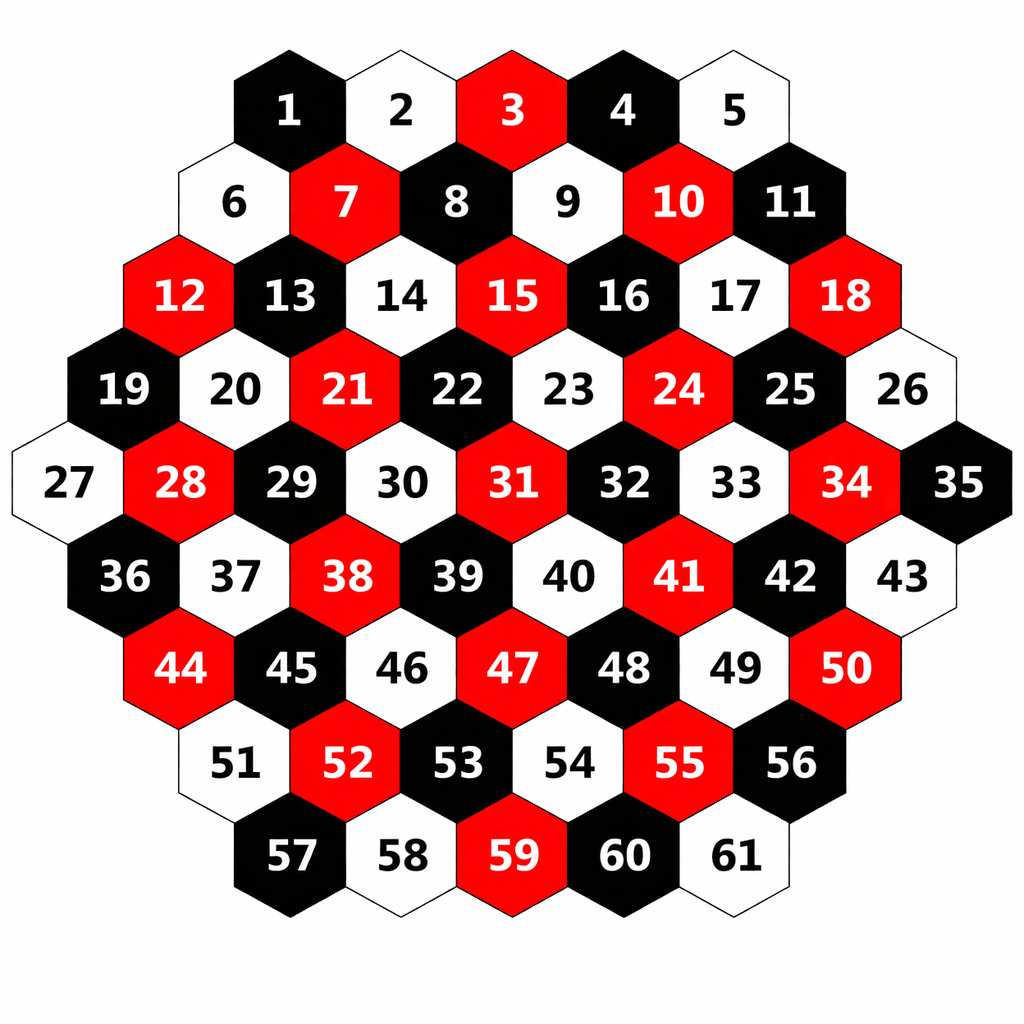
\includegraphics[scale=0.2]{implementation_of_the_game_model/images/numbered_tricolor_board.png}
    \caption{Board with numbered tiles from 1 to 61}
    \label{fig:numbered_tricolor_board}
\end{figure}

Each player starts with 18 pieces, and the number of pieces can only decrease during the game. Therefore, the number of white pieces and the number of black pieces on a tile can each be represented using 5 bits, since values from 0 to 18 must be stored. The owner of a non-empty tile can be represented using 1 additional bit. Empty tiles do not require a separate owner value, since their neutrality can be inferred from the absence of pieces.

In the implemented representation, each tile is stored as a 16-bit integer. The number of white pieces, the number of black pieces, and the owner bit are encoded using bit masks. A visual representation of the board state can be seen in~\ref{fig:board_state_opti}. This compact representation makes it possible to retrieve and modify tile information using bitwise operations, which are efficient and avoid more expensive object-based structures.

\begin{figure}[h]
    \centering
    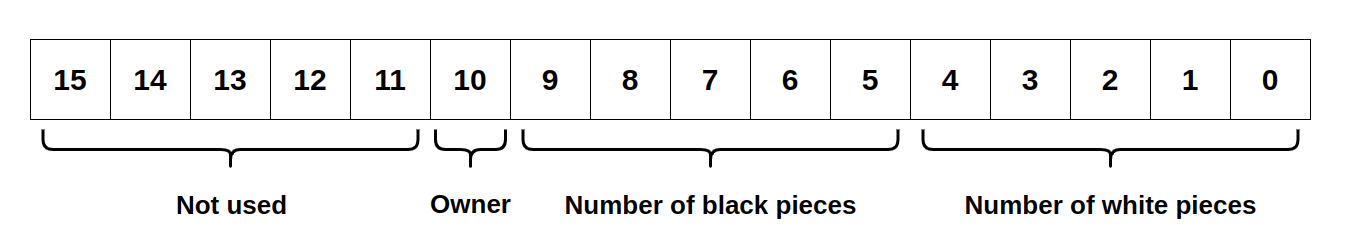
\includegraphics[scale=0.3]{implementation_of_the_game_model/images/board_state_opti.png}
    \caption{16-bit integer visual representation masking the state of the board}
    \label{fig:board_state_opti}
\end{figure}

The player to move is stored separately as a Boolean value. Consequently, the size of a board state is:

%\begin{equation}
   \[ 61 \cdot 16 \text{ bits} + 8 \text{ bits} = 61 \cdot 2 \text{ bytes} + 1 \text{ byte} = 123 \text{ bytes}\]
%    \label{eq:board_state_size}
%\end{equation}

This small memory footprint makes board states inexpensive to copy, which is especially important for search algorithms.

Actions are represented in a similarly compact way. A move in Tricolor is fully described by three pieces of information: the origin tile, the destination tile, and the number of pieces moved. Since the board contains 61 tiles, both the origin and destination indices can be stored using one byte each. The number of moved pieces can also be stored in one byte. An action is therefore represented using only:

%\begin{equation}
   \[ 8 \text{ bits} + 8 \text{ bits} + 8 \text{ bits} = 1 \text{ byte} + 1 \text{ byte} + 1 \text{ byte} = 3 \text{ bytes} \]
%    \label{eq:action_size}
%\end{equation}

This representation is sufficient to apply a move to a board state, while keeping the action structure small enough for efficient storage and manipulation during move generation and search.

\section{Move Generation and Game Simulation}

The move generator is responsible for producing all legal actions available from a given board state. To do this, it first identifies all tiles controlled by the player to move. For each controlled stack, it considers all possible numbers of pieces that may be moved from the top of the stack, all six directions of the hexagonal grid, and all legal distances allowed by the number of friendly pieces in the moving group.

For each candidate movement, the generator verifies the constraints defined in Chapter~\ref{game_rules}. The destination must be reachable in a straight line, and all intermediate tiles must be empty. If the destination tile is empty or controlled by the moving player, the move is legal. If the destination tile is controlled by the opponent, the attacking and defending powers are computed in order to determine whether the move is a capture, an imprisonment, or an illegal move.

The forced-move rule is also handled during move generation. If at least one legal capture or imprisonment is available, then only capture and imprisonment moves are returned as legal actions. Otherwise, all ordinary legal moves are returned. This ensures that agents cannot select moves that violate the rules of Tricolor.

The game simulation loop uses this move generator at each turn. Starting from the initial board position, the current player selects one of the legal actions. The action is then applied to the board state, the current player is updated, and the game checks whether a terminal condition has been reached. A player loses if they have no legal move available on their turn. In addition, the implementation applies the draw condition introduced in Chapter~\ref{game_rules}: if no capture occurs during 100 consecutive turns, the game is declared a draw.

This simulation process is used both for complete games between agents and for internal searches performed by AI algorithms. Its efficiency is therefore central to the experimental results presented in the following chapters.

\section{Agents and User Interface}

Several basic agents were implemented to interact with the game engine.

The Random Agent selects uniformly among the legal actions available in the current position. Although simple, this agent is useful for testing the correctness of the implementation and for generating large numbers of games. It also provides a basic baseline against which stronger agents can later be compared.

The Human Agent allows a human player to select actions manually. This is useful for exploring the game, checking rule behavior in specific situations, and playing against either another human or an AI agent.

A graphical user interface was developed using the SFML library. The interface displays the board, the pieces, and the current position, and allows games to be visualized during play. This visual component is useful not only for human play, but also for debugging and for interpreting the behavior of agents during simulations.

The implementation therefore serves two complementary purposes. It provides an efficient experimental framework for automated simulations and AI search, while also offering a visual tool for exploring Tricolor positions and gameplay. The framework described in this chapter provides the basis for the quantitative analysis of Tricolor presented in the next chapter.

%%%%%%%%%%%%%%%%%%%%%%%%%%%%%%%%%%%%%%%%%%%%
\begin{comment}
The framework for the game \textbf{Tricolor} was implemented in C++. This choice was made because C++ is a low-level language that allows efficient memory management and runtime optimization.

\section{Game Logic}

The game logic refers to the set of low-level structures that must be implemented to model the game Tricolor accurately.

These three structures are:
\begin{itemize}
    \item \textbf{Board State}
    \item \textbf{Actions}
    \item \textbf{Game}
\end{itemize}

\subsection{Board State}

The board state is one of the most important features of the game logic. This is because it must encode all the necessary information required to define a specific state of the board, but also because it needs to be easy to \textit{copy}. For a proper AI analysis of games, being able to make fast copies of any board state is crucial as all modern AI algorithms (e.g. AlphaBeta and MCTS) need to do it hundreds or thousands of times ~\cite{alpha_beta}.

In the search of the most compact board state representation, it's important to have the following insights:
\begin{itemize}
    \item The board has 61 tiles, as you can see in Figure~\ref{fig:numbered_tricolor_board}. Therefore, an array of size 61 can be used, where each element represents one single tile.
    \item Each player starts with 18 pieces (so there are 18 white pieces and 18 black pieces on the board). The number of pieces can't increase, because there is no such feature in the game. However, pieces of the same or different color can be stack on the same tile, which means, in theory, a tile could have 18 white pieces and 18 black pieces. Moreover, when a tile contains mixed colors pieces, it's impossible to deduce what player owns the tile, so it's required to have metadata describing the owner.
    \item It's important to know what player has to make the next move for the current pieces positions on the board.
\end{itemize}

\begin{figure}[h]
    \centering
    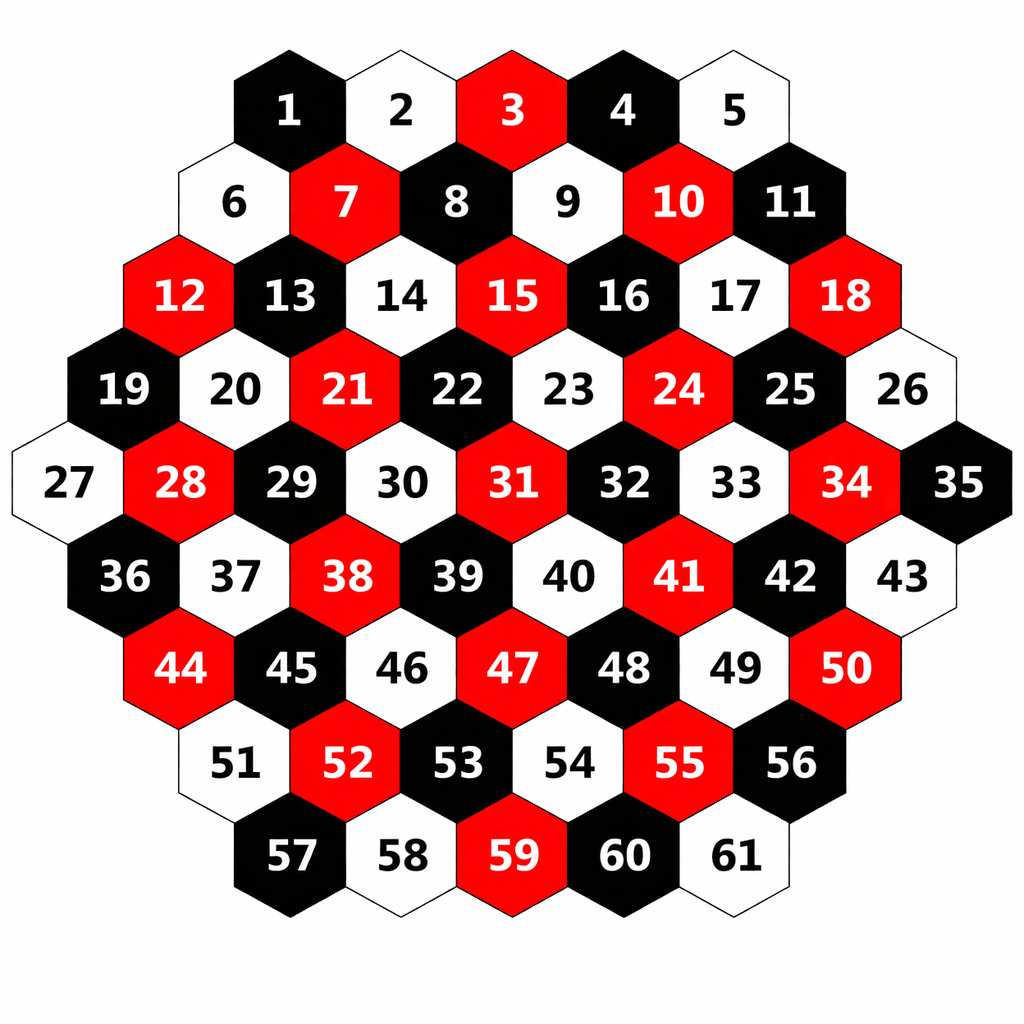
\includegraphics[scale=0.2]{implementation_of_the_game_model/images/numbered_tricolor_board.png}
    \caption{Board with numbered tiles from 1 to 61}
    \label{fig:numbered_tricolor_board}
\end{figure}

With these 3 insights we can conclude that a good data structure for the board state is an array of length 61 (for the number of tiles of the board) where each element is a 16 bits number. This is because, for each tile, we need to maintain the number of white and black pieces (from 0 to 18 for each color, which means we need 5 bits for each color, so 10 bits in total), as well as the owner of the tile (there are only 2 players, so we only need 1 bit; notice that for the neutral tiles, i.e. the empty tiles, it's possible to deduce the owner of the tile by the fact that there are no pieces at all, so no need for a "third" owner). A visual representation of the bit masking of each tile can be seen in Figure~\ref{fig:board_state_opti}. Finally, the player who has to move in the current position is maintained using a boolean value (0 = white has to move and 1 = black has to move).

\begin{figure}[h]
    \centering
    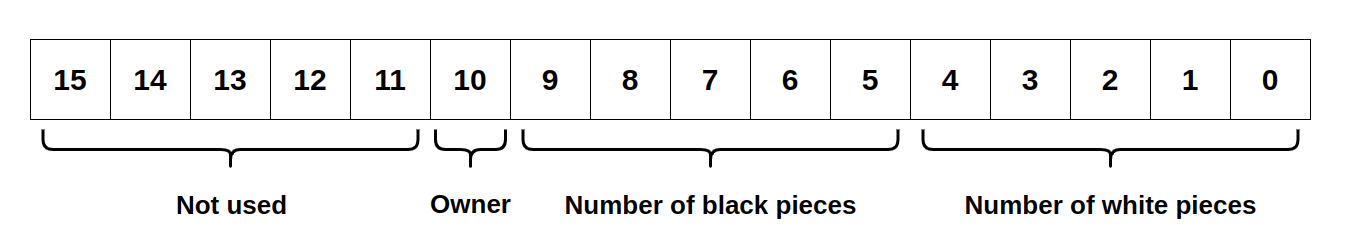
\includegraphics[scale=0.3]{implementation_of_the_game_model/images/board_state_opti.png}
    \caption{16-bit integer visual representation masking the state of a board}
    \label{fig:board_state_opti}
\end{figure}

This final compact structure of a board state has only a size of:
\begin{equation}
61 * 16 \text{ bits} + 8 \text{ bits} = 61 * 2 \text{ bytes} + 1 \text{ byte} = 123 \text{ bytes}
\label{eq:board_state_size}
\end{equation}
, which is really small. Therefore, making a copy of such a state is very fast.

Note: the different operations (getting the number of white pieces, black pieces, owner of a tile etc.) are done only using bitwise operations, making the implementation even faster than a naive one.

\subsection{Actions}

In any game, actions are the bridge between the different board states. In any position, the player that has to make the next move needs a set of actions to choose from (e.g. Player 1 decides to move 3 pieces of this stack to 2 tiles to the left like in Figure~\ref{fig:action_example}). When talking about performance, a model has to:

\begin{enumerate}
    \item generate all the possible actions for a board state as fast as possible
    \item use the least memory possible for the \textbf{action} structure
\end{enumerate}

\begin{figure}[h]
    \centering
    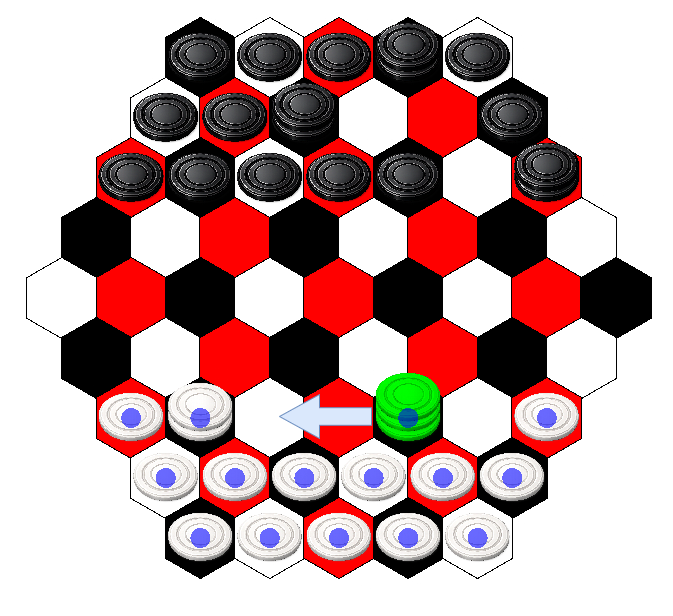
\includegraphics[scale=0.4]{implementation_of_the_game_model/images/action_example.png}
    \caption{Example of the action of Player 1 moving 3 pieces from a stack to 2 tiles to the left}
    \label{fig:action_example}
\end{figure}

Generating all the possible actions for a board state is a straightforward task. It only requires to iterate over all the owned board tiles by the player who's turn is and, depending on the number of pieces on the stack and the surrounding pieces in the 6 directions of the tile, check what actions are possible following the rules of the game described in a previous chapter. There isn't any major optimization that can be brought to this implementation of the actions generation.

For the minimization of memory usage of the \textbf{action} structure, it is sufficient to have the insight that to perfectly describe an action it is only needed to know the \textbf{from} tile, the \textbf{to} tile and the number of pieces moved from the \textbf{from} tile to the \textbf{to} tile. The tiles are numbered from 0 to 60, so 8 bits are sufficient to represent the \textbf{from} and \textbf{to} tiles. A player can theoretically move at most 35 pieces at the same time, so 8 bits are also sufficient to represent the number of moved pieces.

Therefore, the minimal representation of an action has only a size of:
\begin{equation}
8 \text{ bits} + 8 \text{ bits} + 8 \text{ bits} = 1 \text{ byte} + 1 \text{ byte} + 1 \text{ byte} = 3 \text{ bytes}
\label{eq:action_size}
\end{equation}
, which is really small.

\subsection{Game}

Once the Board State and Action structures are implemented, including their useful methods, simulating a game is very simple.

A normal game starts in the position shown in Figure~\ref{fig:board_setup}, where Player 1 (White) has to make the first move. From this point, each player chooses an action on their turn until:
\begin{enumerate}
    \item one of the players has no actions left, resulting in a win for the other player
    \item none of the players captured at least one enemy piece in the last 100 turns, resulting in a draw.
\end{enumerate}

\section{Basic Agents and User Interface}

\subsection{Random Agent}

The most basic and easy to implement "AI" agent is the Random Agent. As its name suggests, the Random Agent chooses every time a random action. It's useful to play and to explore the game using such an agent because:
\begin{itemize}
    \item it is used to analyze the different metrics of the game (e.g. duration,  branching factor etc.).
    \item it is used to test how good other AI agents are. If an AI agent has a 50\% win rate against the Random Agent, it means  it's very bad. However, if the AI agent wins 100\% of the games, it means it's already decent. 
    \item it already creates an opponent who is easy to play against, which gives humans the opportunity to learn basic game strategies.
\end{itemize}

\subsection{Human Agent and User Interface}

The Human Agent is also a basic agent because the action chosen at every turn is the one decided by a human.

To allow human players to compete against other humans or AI agents, a user interface was developed in C++ using the SFML library~\cite{sfml}. SFML is a high-level graphics library that simplifies the implementation of simple 2D games such as Tricolor.

When launching the game, it is needed to specify the two types of agents that will play against each other. The first one is Player 1 (White) and the second one is Player 2 (Black). Then, a window will pop on the screen (see Figure~\ref{fig:game_window}) and the game starts.

\begin{figure}[h]
    \centering
    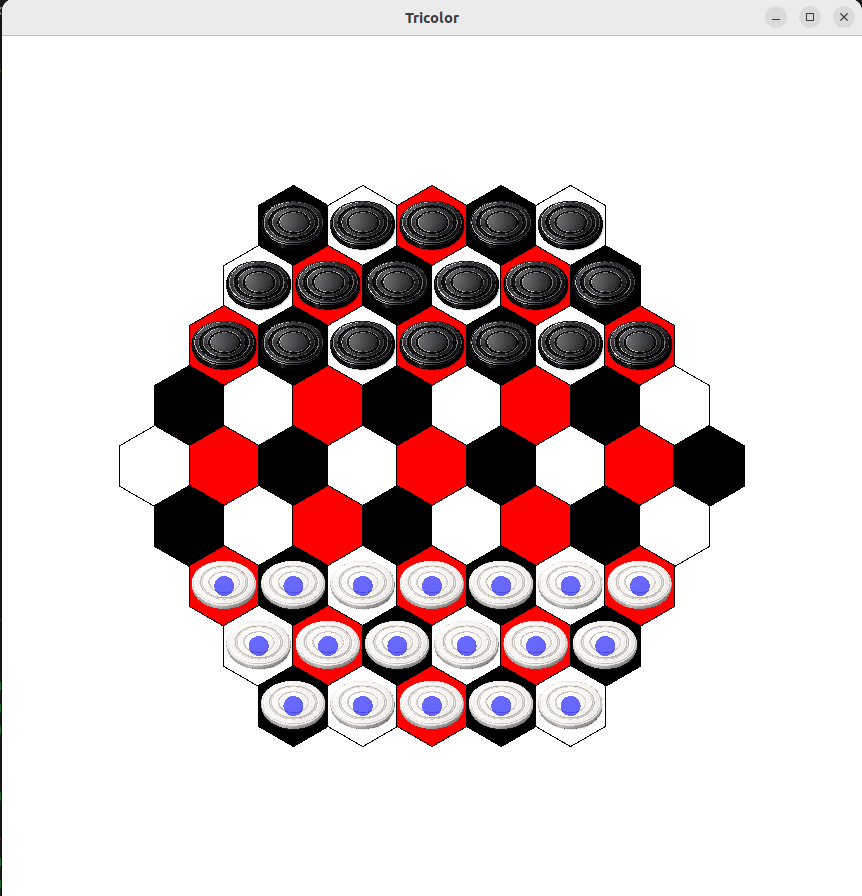
\includegraphics[scale=0.3]{implementation_of_the_game_model/images/game_window.png}
    \caption{Window showing the beginning of a game of Tricolor}
    \label{fig:game_window}
\end{figure}
\end{comment}